\documentclass{article}
\usepackage{caption}
\usepackage{subcaption}
\usepackage{amsmath}
\usepackage{amssymb}
\usepackage[margin=0.75in]{geometry}
\usepackage{fancyhdr}
\usepackage{xcolor}
\usepackage{tikz}
\usepackage[normalem]{ulem} % for strike through text
\setlength{\headheight}{0in}
\newcommand{\Z}{\mathbb{Z}}
\newcommand{\formatVerbalProof}[3]
{
	\noindent{\bf Claim #1:} #2
	\\[0.2cm]\noindent{\bf Proof #1:} #3
}
\newcommand{\formatLogicalProof}[2]
{
	\begin{center}
		\vspace{-0.4cm}
		\begin{tikzpicture}
			\node[rectangle, minimum width=\linewidth, fill=gray!10, draw=gray!50, inner ysep=0.5cm](body1){ #2 };
			\node[anchor=south east](label1) at (body1.south east){\bf Logic for Proof #1};
		\end{tikzpicture}
		\vspace{-0.6cm}
	\end{center}
}
\newcommand{\formatProperties}[2]
{
	\begin{center}
		\vspace{-0.4cm}
		\begin{tikzpicture}
			\node[rectangle, minimum width=\linewidth, fill=gray!10, draw=gray!50, inner ysep=0.5cm, anchor=west](body1){ #2 };
			\node[anchor=south east](label1) at (body1.south east){\bf #1};
		\end{tikzpicture}
		\vspace{-0.6cm}
	\end{center}
}
\newcommand{\formatProof}[4] %#1: proof label. ex: Proof 1-1. #2: proof objective. ex:$R$ must be closed under addition such that $a,b\in R \Rightarrow a\oplus b \in R$. #3 proof (in word form) #4 proof (in logic form)
{
	\formatVerbalProof{#1}{#2}{#3}
	\formatLogicalProof{#1}{#4}
}
\pagestyle{fancy}
\rhead{\today}
\lhead{Daniel Mortensen}
\chead{Homework 2}

\begin{document}
\noindent{\bf Problem 1:} Recall that we discussed number systems by writing an ordered triple $(X, Y, Z)$, where $X$ is a set of things we call `numbers',
$Y$ is the notation for an operation we call `addition', and $Z$ is notation for what we call `multiplication'.
We can do something analogous with \emph{Logical Systems}: we specify the set of statements, the function that determines truth, and the
logical operations and operators.  For the logical system that we (and essentially everyone) use, lets use the notation
$(\mathcal{M}, \Phi, \implies, \wedge, \vee, \neg)$ to mean that $\mathcal{M}$ is the set of statements we work with,
$\Phi$ is the function that assesses truth, and the others are the logical operations and operator.

\vspace{0.1in}\noindent Please prove or disprove that the our logical system $(\mathcal{M}, \Phi, \implies, \wedge, \vee, \neg)$ can be replaced with
$(\mathcal{M}, \Phi, \nabla)$, where $\nabla$ is defined as follows.  For $x, y \in \mathcal{M}$, $x \; \nabla\;y$ is equivalent to
$\neg(x \vee y)$.

\noindent\rule{\textwidth}{0.4pt}\vspace{0.05in}
\noindent{\it Claim: } The logical system $\left (\mathcal{M},\Phi,\implies, \wedge, \vee, \neg \right )$ is equivalent to the logical system $\left( \mathcal{M},\Phi,\nabla \right)$
\\[0.05in] \noindent{\it Proof: } Define an \emph{equivalent system} as one that can express the operators/operations from $(\mathcal{M}, \Phi, \implies, \wedge, \vee, \neg)$ in terms of a new set of operators and operations. In thise case, we desire to show that $\implies, \wedge, \vee, $ and $\neg$ can be expressed in terms of $\nabla$ as defined in the problem statement.
\\[0.1in] \noindent{\it Subclaim 1-1: } The operator $\neg$ can be expressed in terms of $\nabla$.
\\[0.05in]\noindent{\it Subproof 1-1: } Per the definition of $\nabla$ from the problem statement, $p\nabla p \equiv \neg (p \vee p )$. Note that $p \vee p \equiv p$ because \emph{False or False} evaluates to False, and \emph{True or True} evaluates to True as shown in Table \ref{table:truthVee}.
\begin{figure}[h]
\centering
\begin{tabular}{c|c|c}
	$P$ & $Q$ & $P \vee Q$ \\ \hline 
	T   & T   & T \\
	T   & F   & T \\
	F   & T   & T \\
	F   & F   & F \\
\end{tabular}

\caption{Truth Table $\vee$ operator}
\label{table:truthVee}
\end{figure}
Therefore $p\nabla p \equiv \neg \ p$, which implies that the operation $\neg$ can be expressed in terms of $\nabla$. 
\\[0.1in] \noindent{\it Subclaim 1-2: } The operator $\vee$ can be expressed in terms of $\nabla$
\\[0.05in] \noindent{\it Subproof 1-2: } Observe how the truth table for $\vee$ is the converse of the truth table for $\nabla$ as shown in Figure \ref{table:truthVeeAndNabla}, implying that $P\vee Q \equiv \neg(P\nabla Q)$. 
\begin{figure}[h]
\centering
\begin{tabular}{c|c|c}
	$P$ & $Q$ & $P \vee Q$ \\ \hline 
	T   & T   & T \\
	T   & F   & T \\
	F   & T   & T \\
	F   & F   & F \\
\end{tabular} \hspace{0.5in}
\begin{tabular}{c|c|c}
	$P$ & $Q$ & $P \nabla Q$ \\ \hline 
	T   & T   & F \\
	T   & F   & F \\
	F   & T   & F \\
	F   & F   & T \\
\end{tabular} \hspace{0.5in}
\caption{Truth Table for $\vee$ and $\nabla$ operators}
\label{table:truthVeeAndNabla}
\end{figure}
Recall also that the operation $\neg$ can be expressed in terms of $\nabla$ (see Subproof 1-1). By applying the expression for $\neg$ in Subproof 1-1, $P\vee Q$ is shown to be equivalent to $(P\nabla Q)\nabla (P\nabla Q)$. Therefore, the operator $\vee$ can be expressed in terms of $\nabla$.
\\[0.1in]\noindent{\it Subclaim 1-3: } The operator $\wedge$ can be expressed in terms of $\nabla$.
\\[0.05in]\noindent{\it Subproof 1-3: } De Morgan's \sout{Law} Theorem, which states that $\neg (P\wedge Q) \equiv (\neg P)\vee(\neg Q)$ allows us to express the operator $\wedge$ in terms of $\neg$ and $\vee$ as
\begin{equation*}
	\neg (P\wedge Q) \equiv (\neg P)\vee(\neg Q) \implies P\wedge Q \equiv \neg \left [ (\neg P) \vee (\neg Q) \right ]
\end{equation*}
and because $\neg$, and $\vee$ have been shown to have equivalent expressions in terms of $\nabla$ in Subproofs 1-1, and 1-2, then $\wedge$ can also be expressed in terms of $\nabla$. 
\pagebreak
\\[0.1in]\noindent{\it Subclaim 1-4: } The operator $\implies$ can be expressed in terms of $\nabla$.
\\[0.05in]\noindent{\it Subproof 1-4: } The truth table for the $\implies$ operator is defined as
\begin{center}
	\begin{tabular}{c|c|c}
		$P$ & $Q$ & $P \implies Q$ \\ \hline
		T   & T   & T \\
		F   & T   & F \\
		T   & F   & T \\
		F   & F   & T \\
	\end{tabular}.
\end{center}
This proof will use a set inclusion approach to demonstrate which operations are equivalent to $\implies$ and show that the equivalent operations can be expressed in terms of $\nabla$. Let each row of the truth table be expressed as an area in a van diagram. In the image below, the forth row of the truth table is represented by the green area, the second by the red, the third by the blue, and fourth by the intersection of red and blue areas respectively. 
\begin{center}
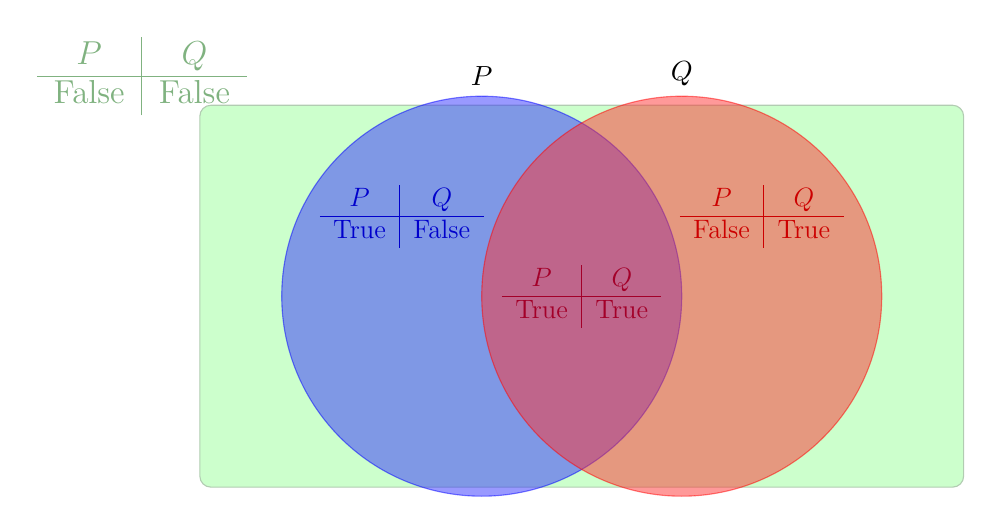
\begin{tikzpicture}
\node[rectangle, rounded corners, draw=green!20!gray!50, minimum width=\textwidth*0.8, minimum height=\textwidth*0.4, fill=green!20] (border) at (0,0) {};
\node[circle, draw, minimum size=2in, color=blue, fill=blue!80, opacity=0.5, label=$P$] (circleA) at (-0.5in,0) {};
\node[circle, draw, minimum size=2in, color=red, fill=red!80, opacity=0.5, label=$Q$] (circleB) at (0.5in,0) {};
\node (text0) at (-2.2in,1.1in){\large\textcolor{green!40!black!50}{\begin{tabular}{c|c}$P$ & $Q$ \\ \hline False & False\end{tabular}}};
\node (text1) at (-0.9in,0.4in){\scalebox{0.8}{\large\textcolor{blue!80!black}{\begin{tabular}{c|c}$P$ & $Q$ \\ \hline True & False\end{tabular}}}};
\node (text2) at (0.9in,0.4in){\scalebox{0.8}{\large\textcolor{red!80!black}{\begin{tabular}{c|c}$P$ & $Q$ \\ \hline False & True \end{tabular}}}};
\node (text3) at (0in,0in){\scalebox{0.8}{\large\textcolor{red!80!blue!80!black}{\begin{tabular}{c|c}$P$ & $Q$ \\ \hline True & True \end{tabular}}}};
\end{tikzpicture}
\end{center}
The truth table for $\nabla$ can be expressed as such as follows:
\begin{center}
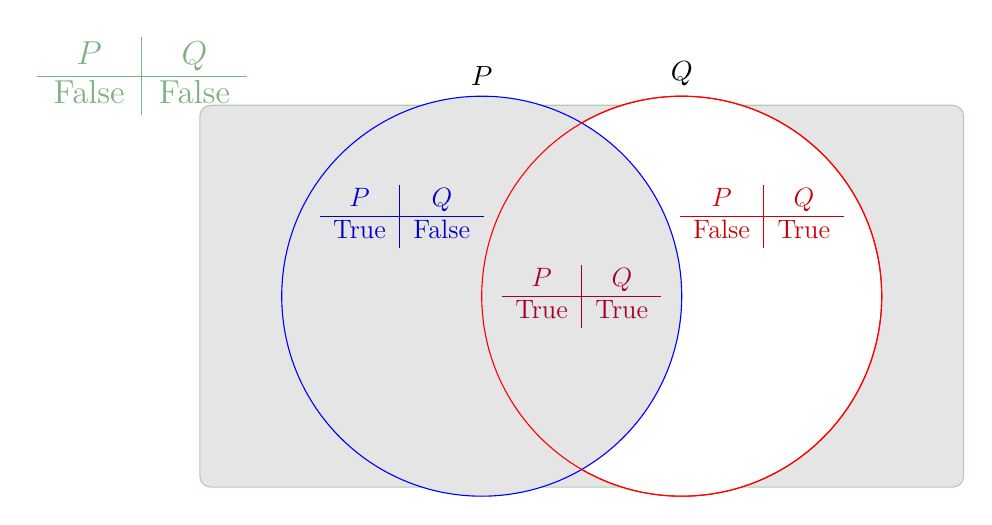
\begin{tikzpicture}
\node[rectangle, rounded corners, draw=green!20!gray!50, minimum width=\textwidth*0.8, minimum height=\textwidth*0.4, fill=gray!20] (border) at (0,0) {};
\node[circle, draw, minimum size=2in, color=red, opacity=1, label=$Q$, fill=white] (circleB) at (0.5in,0) {};
\node[circle, draw, minimum size=2in, color=blue, fill=gray!20, opacity=1, label=$P$] (circleA) at (-0.5in,0) {};
\node[circle, draw, minimum size=2in, color=red, draw opacity=1, fill opacity = 0] (circleB1) at (0.5in,0) {};
\node (text0) at (-2.2in,1.1in){\large\textcolor{green!40!black!50}{\begin{tabular}{c|c}$P$ & $Q$ \\ \hline False & False\end{tabular}}};
\node (text1) at (-0.9in,0.4in){\scalebox{0.8}{\large\textcolor{blue!80!black}{\begin{tabular}{c|c}$P$ & $Q$ \\ \hline True & False\end{tabular}}}};
\node (text2) at (0.9in,0.4in){\scalebox{0.8}{\large\textcolor{red!80!black}{\begin{tabular}{c|c}$P$ & $Q$ \\ \hline False & True \end{tabular}}}};
\node (text3) at (0in,0in){\scalebox{0.8}{\large\textcolor{red!80!blue!80!black}{\begin{tabular}{c|c}$P$ & $Q$ \\ \hline True & True \end{tabular}}}};
\end{tikzpicture}
\end{center}
where the gray regions represent True values in the truth table. The shaded area can be described as ``$P$ or not $Q$'' which translates to the more rigerous statement $P \ \vee \ (\neg Q)$, and has a corresponding truth table of
\begin{center}
	\begin{tabular}{c|c|c}
		$P$ & $Q$ & $P \ \vee \ (\neg Q)$ \\ \hline
		T   & T   & T \\
		F   & T   & F \\
		T   & F   & T \\
		F   & F   & T \\
	\end{tabular}.
\end{center}
The truth table for $P \ \vee \ (\neg Q)$ matches the truth table for the $\implies$ operator.  Additionally, each operator in the statement $P \ \vee \ (\neg Q)$ also has a corresponding counterpart in terms of $\nabla$.  Therefore, the expression $P \ \vee \ (\neg Q)$ also has an expression in terms of $\nabla$, implying that $\implies$ does as well.  
\\[0.1in] Because each operator/operation in the logical system $(\mathcal{M}, \Phi, \implies, \wedge, \vee, \neg)$ can be expressed in terms of $\nabla$, we can say that the logical system $(\mathcal{M}, \Phi, \implies, \wedge, \vee, \neg)$ is equivalent to $(\mathcal{M}, \Phi, \nabla)$.
\\[0.05in] \noindent\rule{\textwidth}{0.4pt}\vspace{0.05in}
\noindent{\bf Problem 2: }Prove that the following game must have a winner.  Place $6$ dots equally spaced on a circle on a piece of paper.
Player A has a red marker and Player B has a blue marker.
Players take turns connecting pairs of dots with line segments using their respective colored markers,
only one line segment between any two dots (therefore at most $15$ line segments will be drawn).
The winner is the first to connect three dots mutually with their respective color, that is, the first to create a monochromatic ``triangle''
in their marker's color.
\noindent\rule{\textwidth}{0.4pt}\vspace{0.05in}
\noindent{\it Claim: } The game given in the problem statement has a winner
\\[0.05in]\noindent{\it Proof: } For the game given in the problem statement to have a winner, all possible outcomes must end in either player blue or player red completing a triangle. This proof uses a subset of the possible edges that connect the six nodes from the game to show that gameplay inevitably results in a triangle. Because the edge subset must occur, then the game will always have a winner. 
\\[0.05in]  Consider the case where one node is connected to three other nodes with edges from the same player as shown in Fig. \ref{fig:problem2a}.
\begin{figure}[h]
\centering
\begin{subfigure}{0.4\textwidth}
\scalebox{0.8}{%
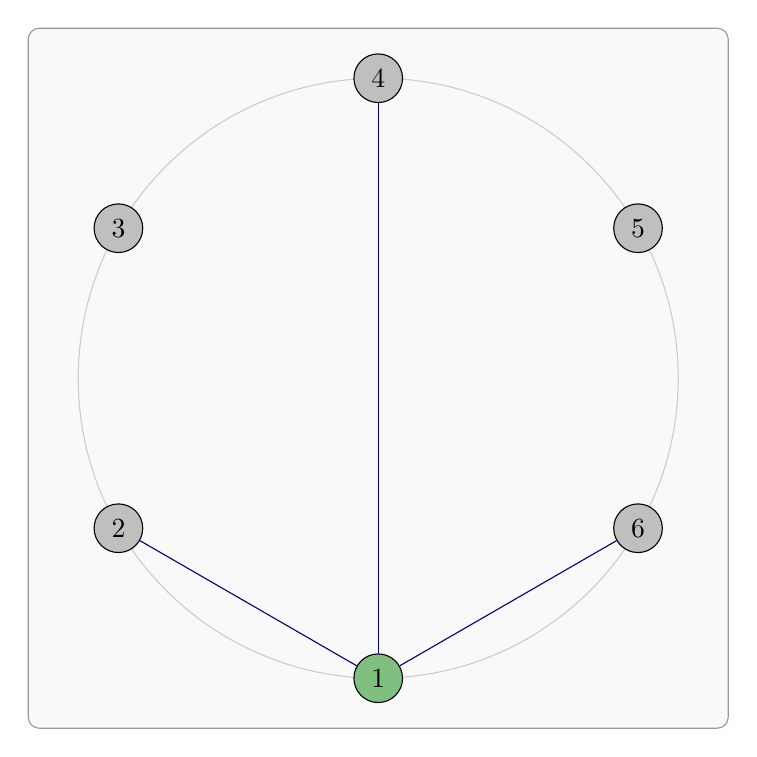
\begin{tikzpicture}
	\node[rectangle, minimum height=3.5in, minimum width=3.5in, fill=gray!5, draw=gray!80, rounded corners] at (0,0){};
	\node[circle, minimum size=3in, draw=black!20] at (0,0)(circle0){};
	\node[circle, minimum size=0.1in, draw=black, fill=gray!50] at (0             ,1.5in     )(circle1){4};
	\node[circle, minimum size=0.1in, draw=black, fill=gray!50] at (1.5in*0.86602 ,1.5in*0.5 )(circle2){5};
	\node[circle, minimum size=0.1in, draw=black, fill=gray!50] at (1.5in*0.86602 ,1.5in*-0.5)(circle3){6};
	\node[circle, minimum size=0.1in, draw=black, fill=green!50!black!50] at (1.5in*0       ,1.5in*-1  )(circle4){1};
	\node[circle, minimum size=0.1in, draw=black, fill=gray!50] at (1.5in*-0.86602,1.5in*-0.5)(circle5){2};
	\node[circle, minimum size=0.1in, draw=black, fill=gray!50] at (1.5in*-0.86602,1.5in*0.5 )(circle6){3};
	\draw[color=black!50!blue](circle4) -- (circle1);
	\draw[color=black!50!blue](circle4) -- (circle3);
	\draw[color=black!50!blue](circle4) -- (circle5);
\end{tikzpicture}
}
\caption{Problem Setup}
\label{fig:problem2a}
\end{subfigure}
\hspace{0.5in}
\begin{subfigure}{0.4\textwidth}
\centering
\scalebox{0.8}{%
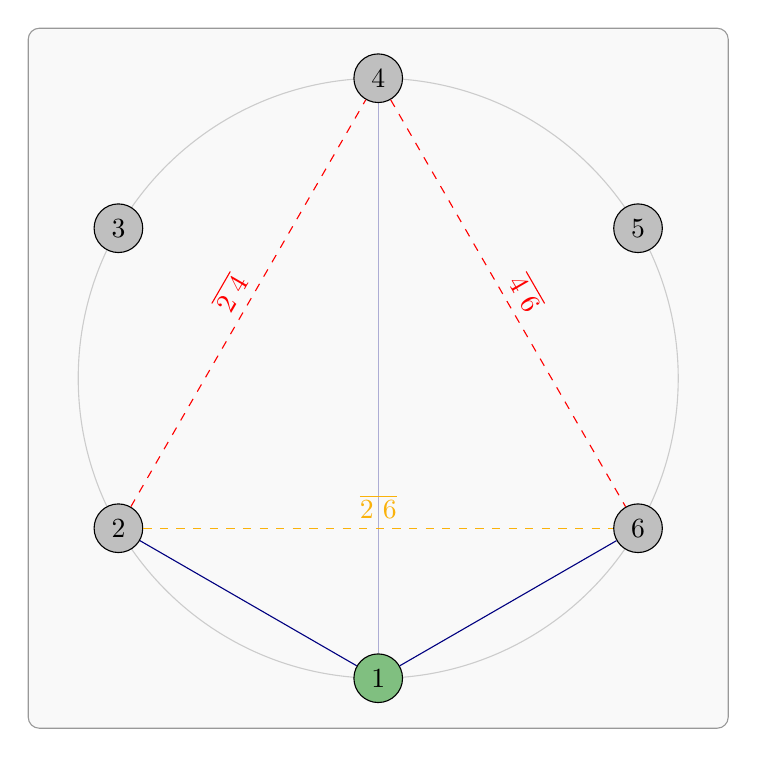
\begin{tikzpicture}
	\node[rectangle, minimum height=3.5in, minimum width=3.5in, fill=gray!5, draw=gray!80, rounded corners] at (0,0){};
	\node[circle, minimum size=3in, draw=black!20] at (0,0)(circle0){};
	\node[circle, minimum size=0.1in, draw=black, fill=gray!50] at (0             ,1.5in     )(circle1){4};
	\node[circle, minimum size=0.1in, draw=black, fill=gray!50] at (1.5in*0.86602 ,1.5in*0.5 )(circle2){5};
	\node[circle, minimum size=0.1in, draw=black, fill=gray!50] at (1.5in*0.86602 ,1.5in*-0.5)(circle3){6};
	\node[circle, minimum size=0.1in, draw=black, fill=green!50!black!50] at (1.5in*0       ,1.5in*-1  )(circle4){1};
	\node[circle, minimum size=0.1in, draw=black, fill=gray!50] at (1.5in*-0.86602,1.5in*-0.5)(circle5){2};
	\node[circle, minimum size=0.1in, draw=black, fill=gray!50] at (1.5in*-0.86602,1.5in*0.5 )(circle6){3};
	\draw[color=black!50!blue, opacity=0.3](circle4) -- (circle1);
	\draw[color=black!50!blue, opacity=1](circle4) -- (circle3);
	\draw[color=black!50!blue, opacity=1](circle4) -- (circle5);
	\draw[dashed, color=red](circle5) -- node[above, sloped]{$\overline{2 \ 4}$}(circle1);
	\draw[dashed, color=red](circle1) -- node[above, sloped]{$\overline{4 \ 6}$}(circle3);
	\draw[dashed, draw=yellow!70!red](circle5) -- node[above, sloped]{\textcolor{yellow!70!red}{$\overline{2 \ 6}$}}(circle3);
\end{tikzpicture}
}
\caption{Edges that ensure a win}
\label{fig:problem2b}
\end{subfigure}
\caption{Visual Aids for Problem 2}
\end{figure}
Suppose there exists a combination of edges that yields no triangles for the current setup. This implies that edges $\overline{2 \ 4}$ and $\overline{4 \ 6}$ must be assigned to player red, but then edge $\overline{2 \ 6}$ will create a triangle for player red or player blue (see Fig. \ref{fig:problem2b}), making either player blue or player red the winner and contradicting the original assumption that there existed a combination which did not yield a winner. The same holds true for cases where one player is assigned four or five edges instead of three as the first three edges are sufficient guarantee a winner. Cases where one player is assigned zero, one or two edges, must also form a triangle because the other player must necessarily be assigned the remaining five, four, or three edges.

\noindent\rule{\textwidth}{0.4pt}\vspace{0.05in}

\noindent{\bf Problem 3: } Prove or disprove that \emph{If $n \in \Z^+$, then $n^2 + n +41$ is prime.}
\\\rule{\textwidth}{0.4pt} 
\\[0.05in]\noindent{\it Claim: If $n \in \Z^+$, then $n^2 + n +41$ is prime.}
\\[0.05in]\noindent{\it Proof: } This proof uses a counter-example to show that the claim is not true as given.  Because $n\in \mathbb{Z}_{+}$, then $n=41$ is a valid value for $n$, but $41^2 + 41 + 41 = 41(41 + 2)$, implying that $\exists k \in \mathbb{Z} \ni k\cdot41 = 41^2 + 41 + 41$. Therefore, when $n=41$, $n^2 + n + 41$ is not prime.
\\[0.05in]\rule{\textwidth}{0.4pt} 
\\[0.05in]\noindent{\bf Problem 4: }Suppose $x$ is a positive integer with $n$ digits, say $x = d_1d_2d_3\cdots d_n$. In other words,
$d_i \in \{0,1,2,\dots, 9\}$ for $1 \leq i \leq n$, but
$d_1 \neq 0$.  Here's a definition: For $a, b \in \Z$, $a$ is a {\bf divisor} of $b$ if $b = ak$, for some $k \in \Z$.
Please prove the following statement: \emph{If $9$ is a divisor of $d_1 + d_2 + \cdots + d_n$, then $9$ is a divisor of $x$.}
\\[0.05in]\noindent{\it Claim: }If $9$ is a divisor of $d_1 + d_2 + \cdots + d_n$, then $9$ is a divisor of $x$.
\\[0.05in]\noindent{\it Proof: } Because $x = d_1d_2d_3\cdots d_n$, $x$ can also be expressed as
\begin{equation*}
	x = d_1\cdot 10^{n-1} + d_2\cdot 10^{n-2} + d_3\cdot 10^{n-3} + \cdots + d_n\cdot 10^{0}.
\end{equation*}
For any power of $10^k$, the largest value that is less than $10^k$ and divisible by $9$ is $10^k - 1$, implying that $\exists a \in \mathbb{Z}_{+} \ni 9a_k + 1 = 10^k$, and consequently that $d_n10^k = 9a_kd_n + d_n$. Therefore, it can be said that 
\begin{equation*}
x = (9a_{n-1}d_1 + d_1) + (9a_{n-2}d_2 + d_2) + (9a_{n-3}d_3 + d_3) + \cdots + (9a_0d_n + d_n),
\end{equation*}
and equivalently that
\begin{equation*}
x = (d_1 + d_2 + d_3 + \cdots + d_n) + 9(a_{n-1}d_1 + a_{n-2}d_2 + a_{n-3}d_3 + \cdots + a_0d_n) .
\end{equation*}
If $9$ is a divisor of $d_1 + d_2 + \cdots + d_n$, then $\exists b \in \mathbb{Z}_{+} \ni 9b = (d_1 + d_2 + d_3 + \cdots + d_n)$, which implies that 
\begin{equation*}\begin{aligned}
x &= 9b + 9(a_{n-1}d_1 + a_{n-2}d_2 + a_{n-3}d_3 + \cdots + a_0d_n) \\
  &= 9(b + a_{n-1}d_1 + a_{n-2}d_2 + a_{n-3}d_3 + \cdots + a_0d_n)
\end{aligned}\end{equation*}
but because $\mathbb{Z}_{+}$ is closed under addition and multiplication, $b + a_{n-1}d_1 + a_{n-2}d_2 + a_{n-3}d_3 + \cdots + a_0d_n \in \mathbb{Z}_{+}$, and therefore, there exists a $c \in \mathbb{Z}_{+} \ni 9c = x$, making $9$ a divisor of $x$. Hence if $9$ is a divisor of $d_1 + d_2 + \cdots + d_n$, then $9$ is a divisor of $x$.
\\[0.05in]\rule{\textwidth}{0.4pt}

\end{document}
